\chapter{Papyrus Project Creation}
\label{sec:Appendix1}

The Papyrus project creation is an important step in the development of DIAs with StreamGen as the UML profile only can be applied when such step is well done. On the other hand, if the process developed along this appendix is required to be replicated, it is important to use the same Eclipse and Papyrus versions. Such versions of Eclipse and Papyrus are specified in the table \ref{Papyrus And Eclipse Versions}.

\begin{table}[h!]
\centering
	\begin{tabular}{||c|c||} 
	\hline\hline
	Program & Version \\ [1ex] 
	\hline\hline
	Eclipse & 2019-03 (4.11.0)  \\
	\hline
	Papyrus & SysML 1.4 Feature 1.3.0  \\
	\hline\hline
	\end{tabular}
\caption{Papyrus And Eclipse Versions}
\label{Papyrus And Eclipse Versions}
\end{table}

Furthermore, before creating the Papyrus project, it is important to import the StreamGen project in the Eclipse workspace.

\section{StreamGen Project Import}

In order to import the StreamGen project in the Eclipse workspace, first of all the File tab must be opened and, then, Open Projects from File System must be clicked. The figure \ref{fig:Import StreamGen Project I} shows the window that is opened once Open Projects from File System is clicked. After such windows is opened, the Directory tab must be clicked and the StreamGen project must be looked for. Once the StreamGen project is imported as a source, the window can be closed by clicking on Finish (figure \ref{fig:Import StreamGen Project II}).

\begin{figure}
\centering
{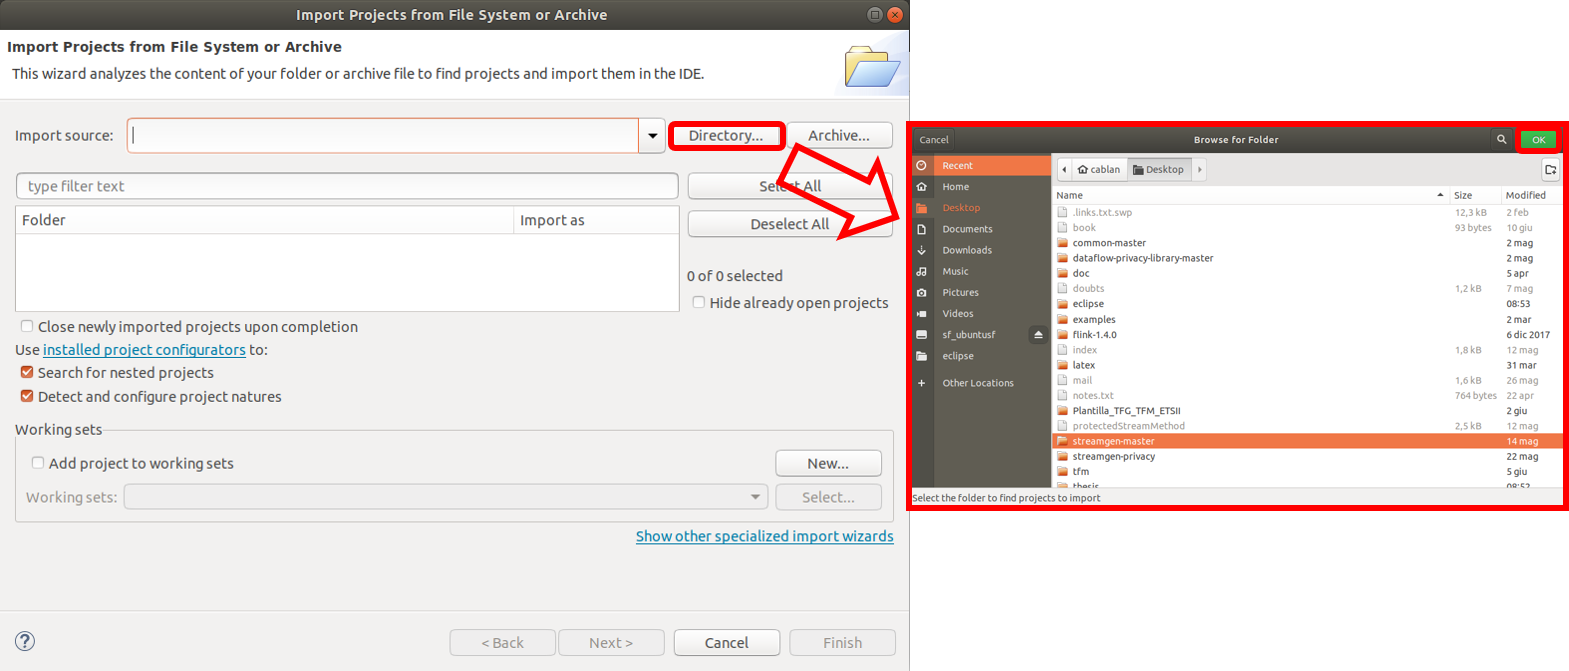
\includegraphics[scale=0.5]{./chapter4/projPapyrus/streamGenImport1.png}}
\caption{Import StreamGen Project I}
\label{fig:Import StreamGen Project I}
\end{figure}

\begin{figure}
\centering
{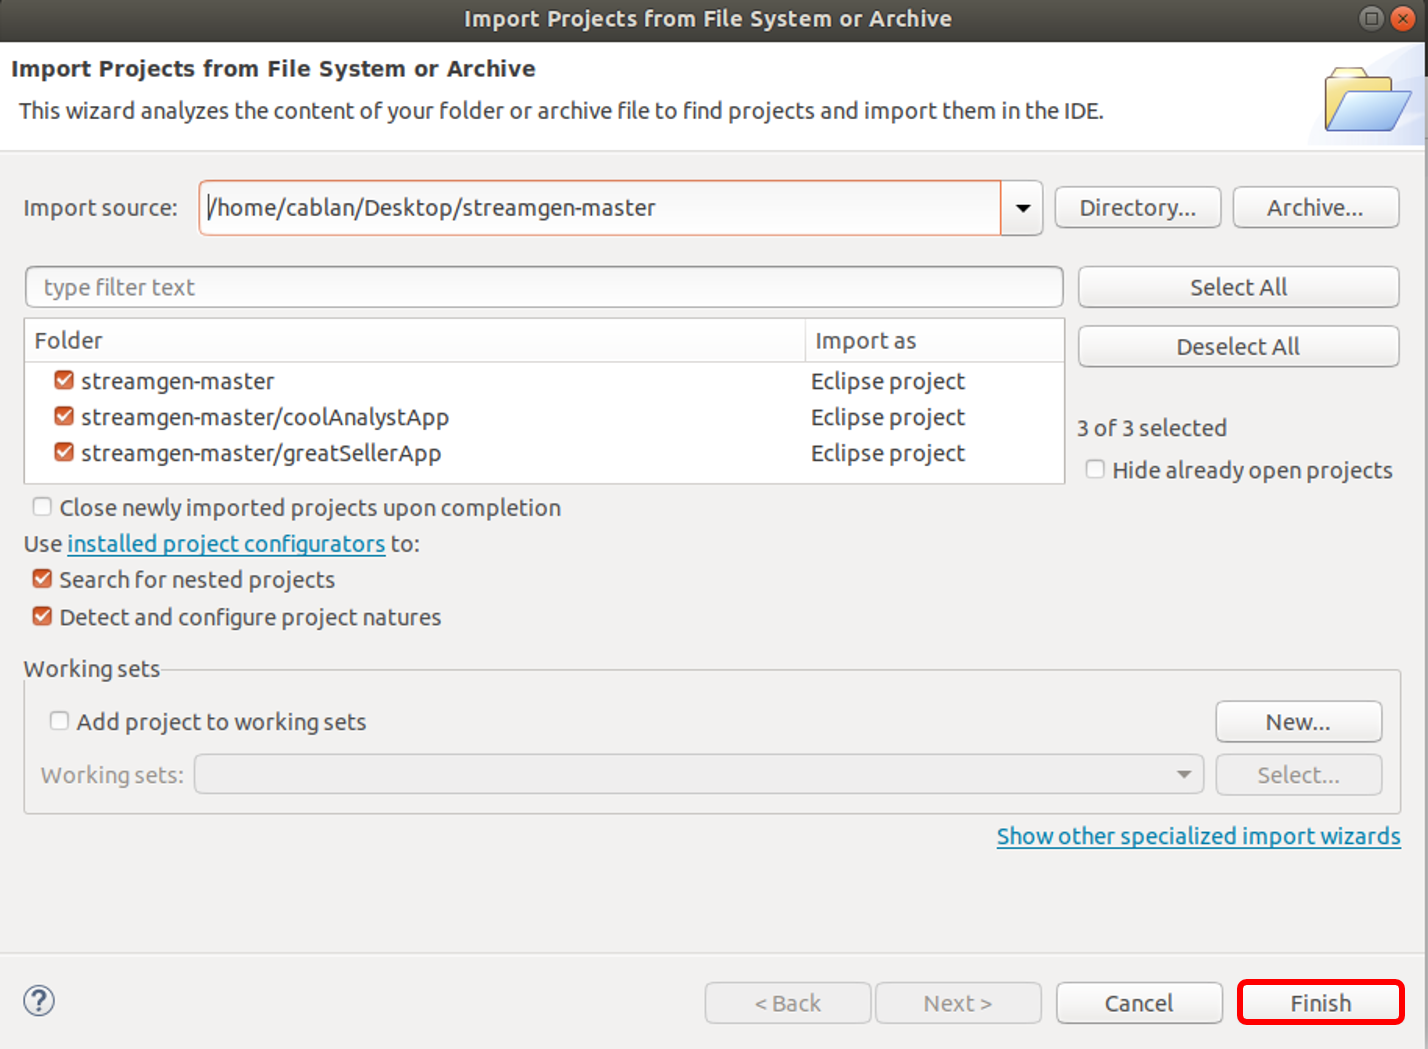
\includegraphics[scale=0.5]{./chapter4/projPapyrus/streamGenImport2.png}}
\caption{Import StreamGen Project II}
\label{fig:Import StreamGen Project II}
\end{figure}

\section{Project Creation Process}

In order to create a Papyrus project with the aim of generating a new DIA with StreamGen, first of all, a new project has to be created in Eclipse. This project is going to be a Papyrus project. In the figure \ref{fig:Papyrus Project} can be seen how a Papyrus project is created in Eclipse once the Papyrus plug in is already installed.

\begin{figure}
\centering
{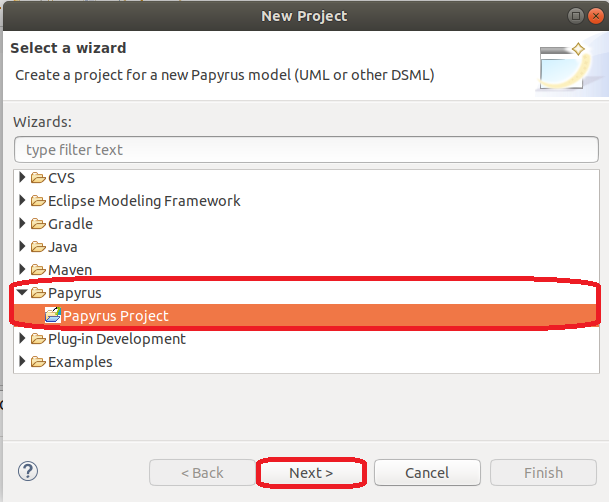
\includegraphics[scale=0.5]{./chapter4/projPapyrus/Selection_001.png}}
\caption{New Papyrus Project}
\label{fig:Papyrus Project}
\end{figure}

Once it is specified in Eclipse that the new project must be a Papyrus project, the Architecture Context of the project has to be specified. Such step is pretty easy as the default values that provides Eclipse are the right ones due to the fact that an UML model is what is required to implement with Papyrus. The figure \ref{fig:Architecture Context} shows a screenshot of the Architecture Context windows and the default values that must be selected in order to generate the Papyrus project with the aim to use StreamGen.

\begin{figure}
\centering
{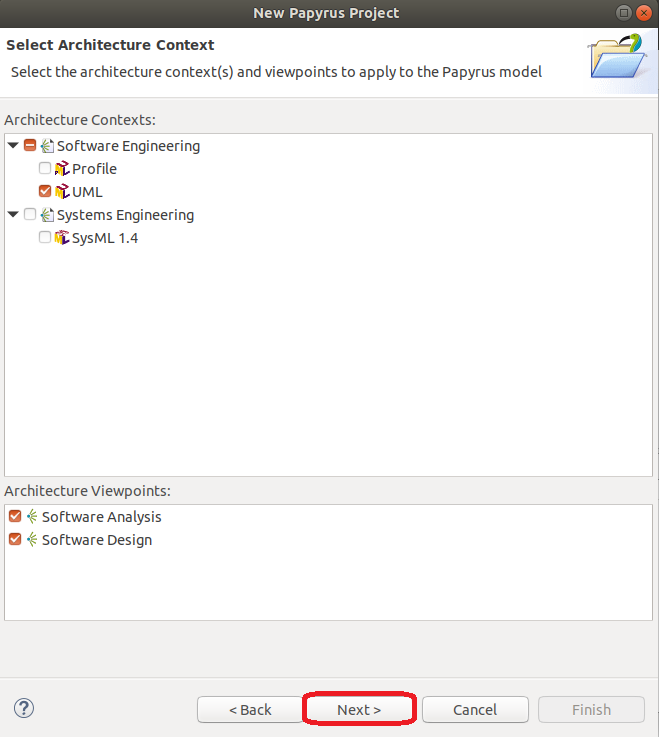
\includegraphics[scale=0.5]{./chapter4/projPapyrus/Selection_002.png}}
\caption{Architecture Context}
\label{fig:Architecture Context}
\end{figure}

After that, the name of the project has to be defined. Due to the fact that it is going to implement an application called Great Seller and Cool Analyst, the name of the Papyrus project is going to be greatSellerApp and coolAnalystApp (figure \ref{fig:Project Name Definition}). In this step any name is allowed, however, it is better to use a name which has sense with the purpose of the application.

\begin{figure}
\centering
{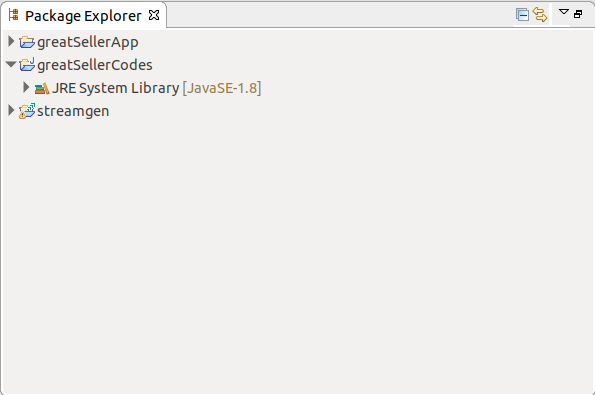
\includegraphics[scale=0.5]{./chapter4/projPapyrus/Selection_003.png}}
\caption{Project Name Definition}
\label{fig:Project Name Definition}
\end{figure}

The next step is to select the representation kind which is the required UML diagram for the development of the DIA and to choose the StreamGen profile as an applied profile of the Papyrus project. In order to develop a DIA, StreamGen requires Papyrus to make a class diagram representation. This is why class diagram is selected in the representation kind field. Moreover, in this step it is assumed that the StreamGen project is already imported in the Eclipse workspace. Then, the profile can be found just browsing in the workspace (streamgen/profile/StreamUML.profile.uml), as it can be seen in the figure \ref{fig:Representation Kind}.

\begin{figure}
\centering
{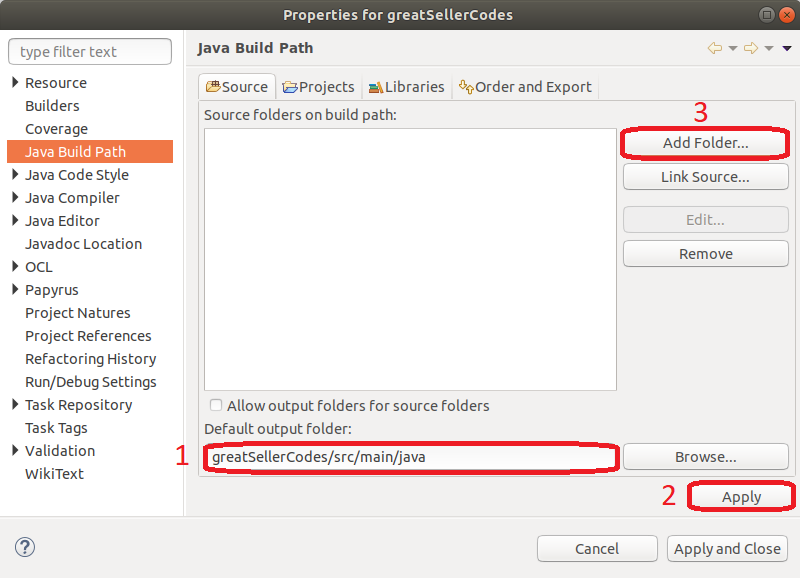
\includegraphics[scale=0.5]{./chapter4/projPapyrus/Selection_004.png}}
\caption{Representation Kind}
\label{fig:Representation Kind}
\end{figure}

Finally, once the StreamGen profile is already selected as a profile to be applied, the Papyrus project creation can be finished just pressing on Finish as it is shown in the figure \ref{fig:Papyrus Project Definition}.

\begin{figure}
\centering
{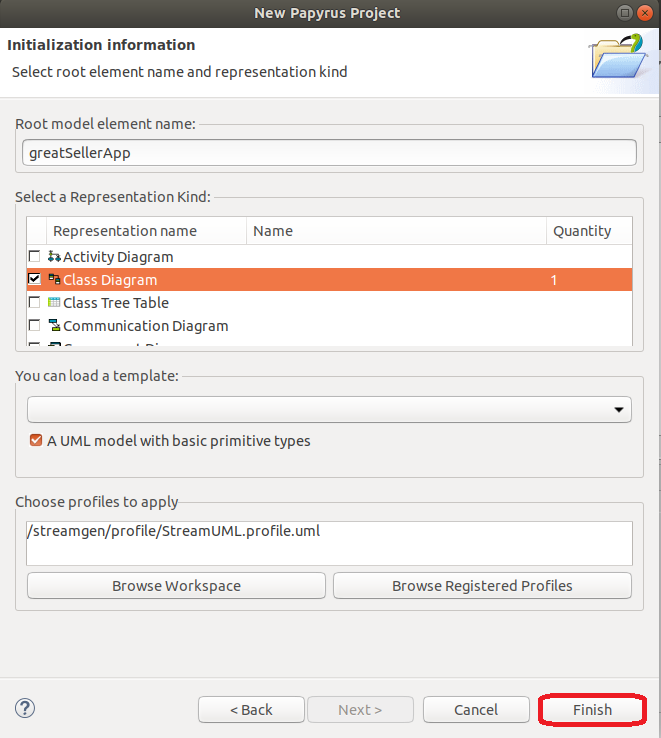
\includegraphics[scale=0.5]{./chapter4/projPapyrus/Selection_005.png}}
\caption{Papyrus Project Definition}
\label{fig:Papyrus Project Definition}
\end{figure}
